\section{Numerical Results}

Currently, the Python package DLRBniCSx facilitates the creation of ANN-POD-based models for solving different types of partial differential equations. While the package currently integrates PyTorch for ANN functionality, a significant aspect of this project involves extending support for TensorFlow within DLRBniCSx. This expansion encompasses various aspects such as model construction, training-validation, data preprocessing, and auxiliary functionalities like error analysis. Further information regarding these enhancements can be found on the project's GitHub page.

\subsection{Effectiveness of POD}

Recall that in Section 4, we compared the choices of parameterisation through the POD results in both cases. In the first scenario, we varied only two parameters ($\mu_1$ and $\mu_2$), with each parameter taking on 10 values. This configuration yielded a total of 100 solutions for POD. In the second scenario, we explored all five parameters, each taking $4 \times 4 \times 3 \times 3 \times 3$ values. This resulted in a larger dataset consisting of 432 solutions for POD. In both cases, we set $N_{max} = 20$ and $\epsilon = 10^{-4}$ as the stopping criterion \footnote{see Section 4.1 for details}.


\begin{figure}[!h]
    \centering
    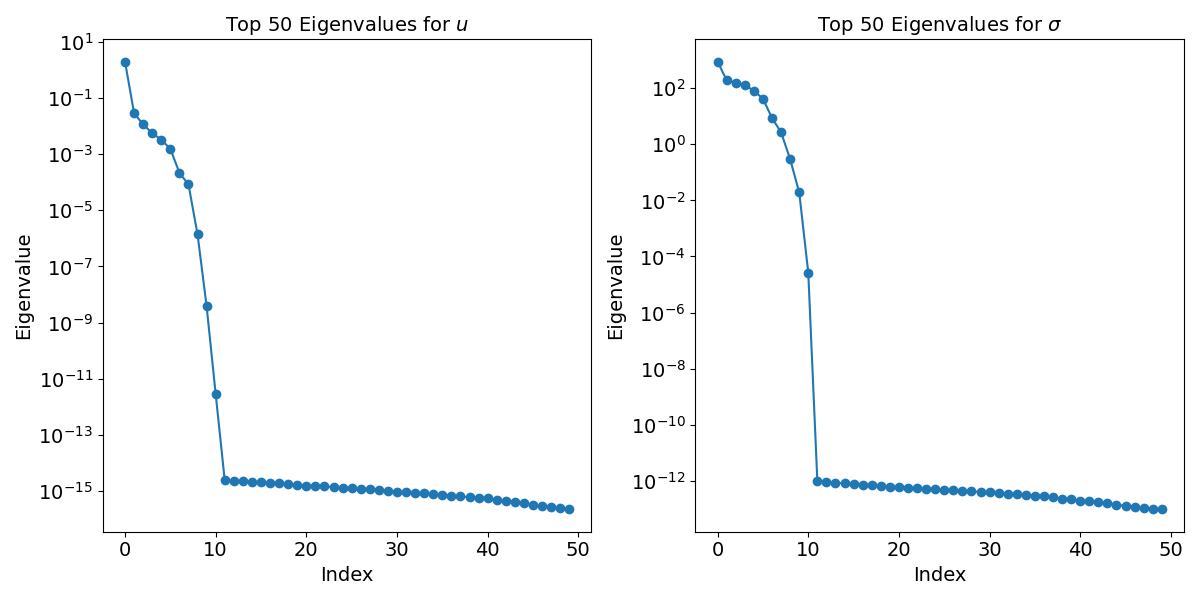
\includegraphics[width=0.8\linewidth]{fig_pod/eigendecay_10,10.png}
    \caption{Top 50 Eigenvalues from POD with varying $\mu_1$ and $\mu_2$, each parameter spanning 10 discrete values}
    \label{fig:eigendecay_10by10}
\end{figure}

\begin{figure}[!h]
    \centering
    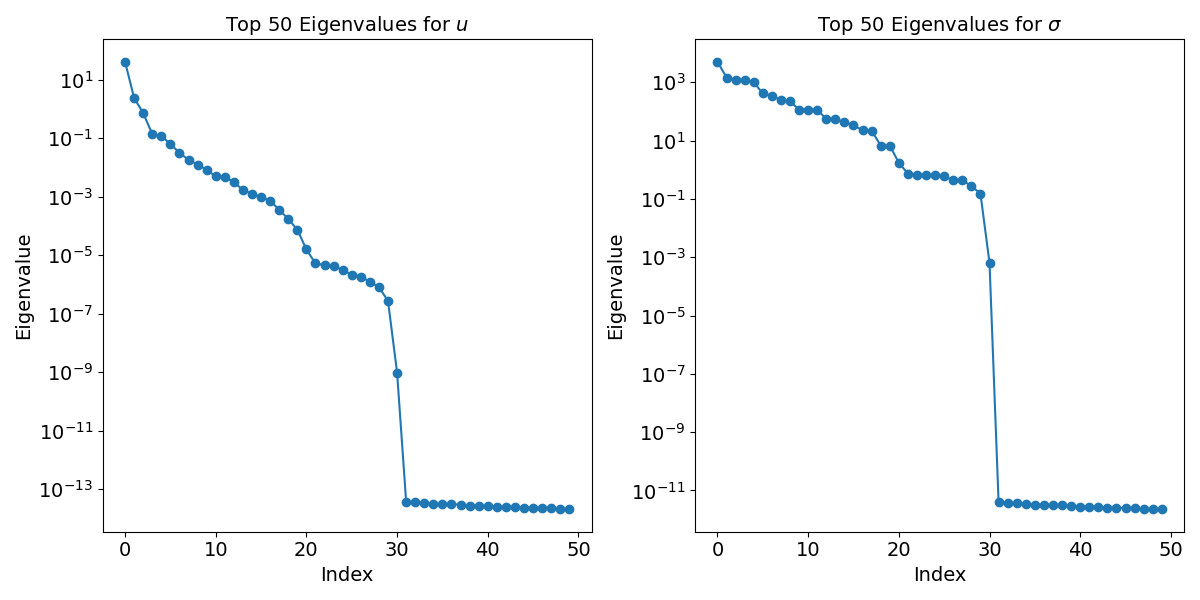
\includegraphics[width=0.8\linewidth]{fig_pod/eigendecay_4,4,3,3,3.png}
    \caption{Top 50 Eigenvalues from POD with varying all parameters, with $\mu_1$ and $\mu_2$ spanning 4 discrete values, $\mu_3$, $\mu_4$ and $\mu_5$ each spanning 3 discrete values}
    \label{fig:eigendecay_allvary}
\end{figure}

 Table \ref{tab:POD_results} compares the proposed two cases, where we can observe that the reconstruction error for both $u$ and $\sigma$  were greatly reduced with only 2 parameters and the size of the reduced basis space despite a much lower number of solutions used. Note that for $\sigma$ in the 5-parameter case, the size of the reduced basis was even reaching the maximum threshold $N_{max}$, meaning that ideally we still need more modes to capture the features of the solutions. 

\begin{table}[htb]
    \centering
    \caption{Results of POD and reconstruction on different parameter sets}
    \begin{tabular}{l|l|l}
        \toprule
        \textbf{Number of Parameters} & 2 & 5 \\
        \midrule
        \textbf{Sample Size} & $10 \times 10$ & $4 \times 4 \times 3 \times 3 \times 3$\\
        \textbf{Size of $\mathbf{V}_{rb}$ ($u$, $\sigma$)} & (7, 9)  & (14, 20) \\
        \textbf{Mean Error ($u$, $\sigma$)} & (0.012, 0.005) & (0.062, 0.246) \\
        \textbf{Max Error ($u$, $\sigma$)} & (0.067, 0.015) & (0.293, 0.781) \\
        \textbf{POD Time in Seconds ($u$, $\sigma$)} & (30, 240) & (2, 13) \\
        \bottomrule
    \end{tabular}
    \label{tab:POD_results}
\end{table}

 Figure \ref{fig:eigendecay_10by10} shows the decay of eigenvalues when performing SVD on the snapshot matrix, varying $\mu_1$ and $\mu_2$, each parameter spanning 10 discrete values (total 100 combinations). Figure \ref{fig:eigendecay_allvary} shows the decay of eigenvalues when varying all parameters, with the number of values for $\bm{\mu}$ equals $[4,4,3,3,3]$ (total 432 combinations). The eigenvalues for both  $u$ and $\sigma$ decay very quickly with only 2 varying parameters, while taking much longer for the 5-parameter case. This also corresponds to the fact that a higher number of reduced basis functions was needed.  

Further to the accuracy of POD, the computational efficiency of the POD process is also greatly hindered by the high number of training snapshots needed with more parameters. Due to the nature of the snapshot matrix being a dense matrix, it was impossible to parallelise the process across multiple CPU cores, so the POD process would take a long time in serial. Tabel \ref{tab:POD_results} proved this point as the POD time for 2 parameters was less than 10\% than that for 5 parameters, and this was even excluding the time for generating the solution snapshot matrix. In addition, a higher number of reduced basis sizes would also incur additional costs in projecting the high-fidelity solution onto the reduced basis space. This proved to be particularly costly as we later tried to initialise the training inputs for the ANN, which required a large amount of data points.

These results have justified our choices of parameterisations on $[\mu_1, \mu_2]$ only, which ensured the numerical stability of the results. A further enhancement was made by reducing the tolerance for retained energy of POD to $\epsilon = 10^{-6}$. This further brought the POD error down by an order of 10, while only introducing an additional reduced basis size for both $u$ and $\sigma$, which we believe is worth the trade-off, as shown by the results presented in table \ref{tab:POD_results_different_epsilon}

\begin{table}[htb]
    \centering
    \caption{Results of POD reconstruction with different $\epsilon$, sample size = $10 \times 10$}
    \small
    \begin{tabular}{c|c|c|c}
        \toprule
        $\epsilon$ & Size of $\mathbf{V}_{rb}$ ($u$, $\sigma$) & Mean Error ($u$, $\sigma$) & Max Error ($u$, $\sigma$) \\
        \midrule
        $10^{-4}$ & (7, 9) & (0.012, 0.005) & (0.067, 0.015) \\
        $10^{-6}$ & (8, 10) & ($8.6 \times 10^{-4}$, $3.5 \times 10^{-4}$) & (0.0028, 0.0023)  \\
        \bottomrule
    \end{tabular}
    \label{tab:POD_results_different_epsilon}
\end{table}

All the results above were recorded based on the case where we employed a general parameter range where $\mu_1 \in [5, 20]$ and $\mu_2 \in [10, 20]$. Although we, later on, chose a different range because of the ANN accuracy, they still served the purpose of selecting the suitable number of parameters and $\epsilon$. Tuning the parameter range of interest to $\mu_1 \in [2\pi, 2.5\pi]$ and $\mu_2 \in [12, 13]$ after we studied the results for the ANN model, the POD results are presented below in table \ref{tab:POD_results_final_range}:

\begin{table}[htb]
    \centering
    \caption{Results of POD reconstruction with $\mu_1 \in [2\pi, 2.5\pi]$, $\mu_2 \in [12, 13]$ and $\epsilon = 10^{-6}$}
    \small
    \begin{tabular}{c|c|c|c}
        \toprule
        Sample Size & Size of $\mathbf{V}_{rb}$ ($u$, $\sigma$) & Mean Error ($u$, $\sigma$) & Max Error ($u$, $\sigma$) \\
        \midrule
        $10 \times 10$ & (4, 4) & ($3.3 \times 10^{-4}$, $8.3 \times 10^{-4}$) & ($7.3 \times 10^{-4}$, $2.20 \times 10^{-3}$) \\
        \bottomrule
    \end{tabular}
    \label{tab:POD_results_final_range}
\end{table}

\subsection{Effectiveness of ANN}


\vspace{1cm}
\#\#\#\#\#\#\#\#\#\#\#\#\#\#\#\#\#\#\#\#\#\#\#\#\#\#\#\#\#\#\#\#\#\#\#\#\#\#\#

\textcolor{red}{Serial: Include training time and data generation time, snapshot computation time for POD, POD process time, eigenvalue decay, loss wrt to epochs for ANN, projection error and ANN error
Snapshot computation time in parallel, with different solvers (not main focus of work)}


Add a ANN sample figure with input and output shape represented

Model Description, discussions on layers and number of neurons, activation functions and maybe stopping criteria. 


Final results for a sigmoid activation function with 500 training and validation samples:
Mean error for U is: 0.398826; Mean Error for SIGMA is 0.862105
Maximum error for U and SIGMA are: 0.771895, 0.999538

Final results for a sigmoid activation function with 1000 training and validation samples: (mu1 and mu2 only)
Mean error for U is: 0.147512; Mean Error for SIGMA is 0.252696
Maximum error for U and SIGMA are: 0.582387, 0.605089

Final results for a sigmoid activation function with 1000 training and validation samples: 
Mean error for U is: 0.102683; Mean Error for SIGMA is 0.248321
Maximum error for U and SIGMA are: 0.553261, 0.813254

Final results for a sigmoid activation function with 500 training and validation samples:
Learing rate = 0.002, ANN structure = [20, 20]
Mean error for U is: 0.055362; Mean Error for SIGMA is 0.152036
Maximum error for U and SIGMA are: 0.163079, 0.442326


Activation: sigmoid
Learing rate = 0.003, ANN structure = [25, 25]
Mean error for U is: 0.066273; Mean Error for SIGMA is 0.140492

(MSE for u, MAE for sigma)
Final results for a sigmoid activation function with 500 training and validation samples:
Learing rate = 0.002, ANN structure = [20, 20]
Mean error for U is: 0.081644; Mean Error for SIGMA is 0.167260
Maximum error for U and SIGMA are: 0.240615, 0.388974
Maximum error for U and SIGMA are: 0.212036, 0.228014

(MSE for both)
Final results for a sigmoid activation function with 500 training and validation samples:
Learning rate = 0.0025, ANN structure = [20, 20]
Mean error for U is: 0.090378; Mean Error for SIGMA is 0.304891
Maximum error for U and SIGMA are: 0.278097, 0.787646;

MSE for both
Final results for a tanh activation function with 400 training and validation samples:
Learing rate = 0.0005, ANN structure sigma:[15, 15], u: [25, 25]
Mean error for U is: 0.025661; Mean Error for SIGMA is 0.026224
Maximum error for U and SIGMA are: 0.043447, 0.069763

Final results for a tanh activation function with 200 training and validation samples:
Learing rate = 0.0005, ANN structure sigma:[15, 15], u: [25, 25]
Mean error for U is: 0.026253; Mean Error for SIGMA is 0.075967
Maximum error for U and SIGMA are: 0.048862, 0.110272
\#\#\#\#\#\#\#\#\#\#\#\#\#\#\#\#\#\#\#\#\#\#\#\#\#\#\#\#\#\#\#\#\#\#\#\#\#\#\#


final loss from each model
effect of the number of training parameters
effect of learning rate and optimisers
final prediction norm error